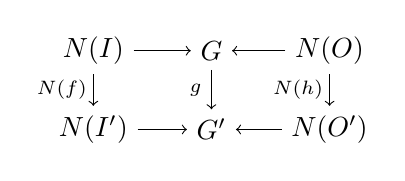
\begin{tikzpicture}
\node (v1) at (1,0) {$N(I)$};
\node (v3) at (2.5,0) {$G$};
\node (v5) at (4,0) {$N(O)$};
\node (v2) at (1,-1) {$N(I')$};
\node (v4) at (2.5,-1) {$G'$};
\node (v6) at (4,-1) {$N(O')$};
\node at (0.6,-0.5) {\scriptsize $N(f)$};
\node at (2.3,-0.5) {\scriptsize $g$};
\node at (3.6,-0.5) {\scriptsize $N(h)$};
\draw [->]  (v1) edge (v2);
\draw [->] (v3) edge (v4);
\draw [->] (v5) edge (v6);
\draw [->] (v1) edge (v3);
\draw [->] (v2) edge (v4);
\draw [->] (v5) edge (v3);
\draw [->] (v6) edge (v4);
\end{tikzpicture}